\documentclass[UTF8,a4paper,12pt]{ctexart}
\usepackage[a4paper,margin=2.2cm]{geometry}
\usepackage{graphicx,float,booktabs,longtable,xcolor,listings,hyperref}
\hypersetup{colorlinks=true,linkcolor=blue,urlcolor=blue}
\setlength{\parindent}{2em}\setlength{\parskip}{0.45em}\sloppy
\newcommand{\shot}[2]{\begin{figure}[H]\centering\includegraphics[width=0.96\textwidth]{截图/#1}\caption{#2}\end{figure}}
\title{计算机网络技术实践实验六报告\\\large Cisco、Juniper与H3C综合互联设计}
\author{学号：已隐去}
\date{2026年10月15日}
\begin{document}\maketitle
\begin{abstract}本实验完成了三厂商拓扑、配置生成、只读远端验收工具和Cisco功能预演。Cisco预演有通过证据，但真实Juniper/H3C设备和端点缺失，因此不能宣称三厂商实验完成。\end{abstract}
\section{实验要求与目标}
实验六要求在一个综合网络中互联Cisco、Juniper和H3C，并验证动态路由学习、远端LAN路由和多台PC互ping。我们把配置生成、远端只读验收和Cisco功能预演分开，避免把单一厂商模拟结果伪装成三厂商结果。
\section{自有拓扑与地址规划}
设计包含4台路由器和8台PC。transit共享网段使用205.161.255.0/24，四个路由器LAN分别使用205.161.1.0/24至205.161.4.0/24，LAN网关尾号254。R1为Juniper、R2为Cisco、R3/R4为H3C；现场接口名称需按实际设备确认。
\begin{figure}[H]\centering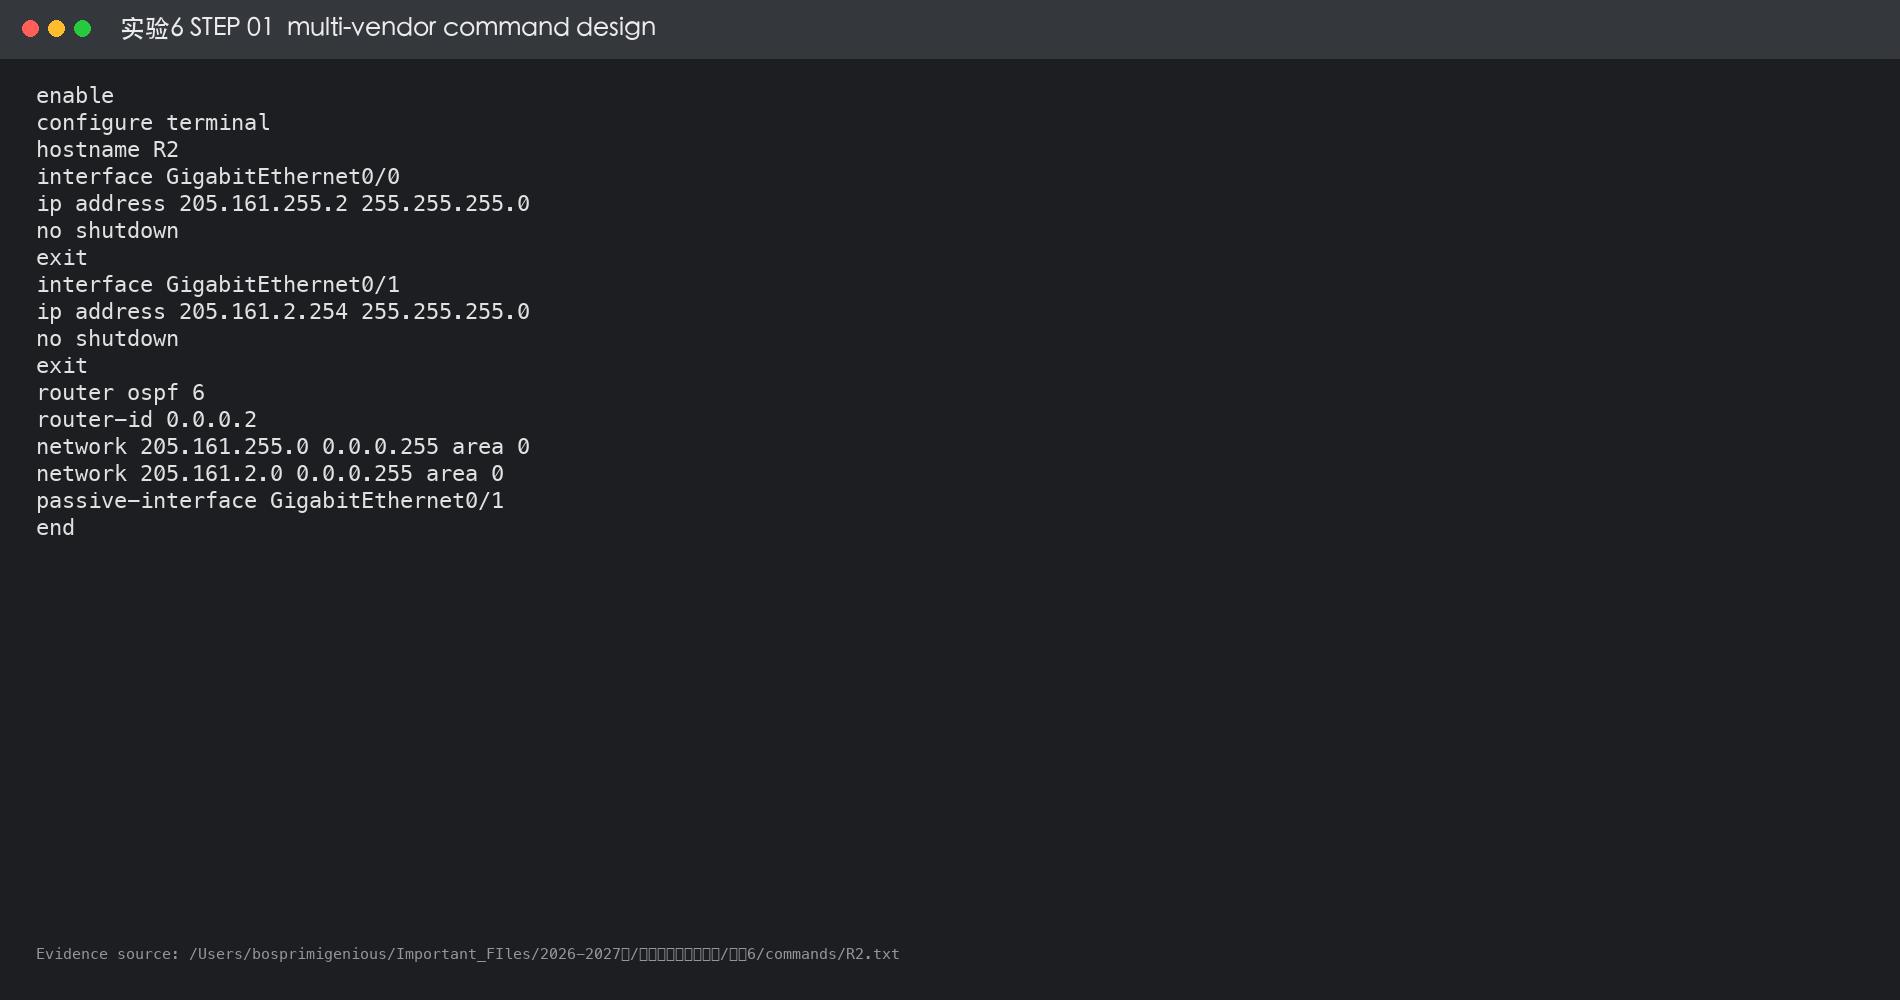
\includegraphics[width=0.96\textwidth]{截图/01-配置生成.png}\caption{自有多厂商配置命令示例。}\end{figure}
\section{配置生成与验收方法}
generate.py从topology.json生成各厂商命令，覆盖保护避免误写已有内容。真实验收工具只读采集version、接口、邻居、路由和PC互ping，不保存密码、不自动改写设备。真实端点文件必须由实验室设备信息填充。
\section{Cisco功能预演}
cisco-proxy使用本地Cisco IOS模拟4路由器、8PC和OSPF，检查3条远端路由、邻居和56方向互ping，并采集OSPF/ICMP。预演用于验证地址规划和验收逻辑，不能替代Juniper/H3C。
\begin{figure}[H]\centering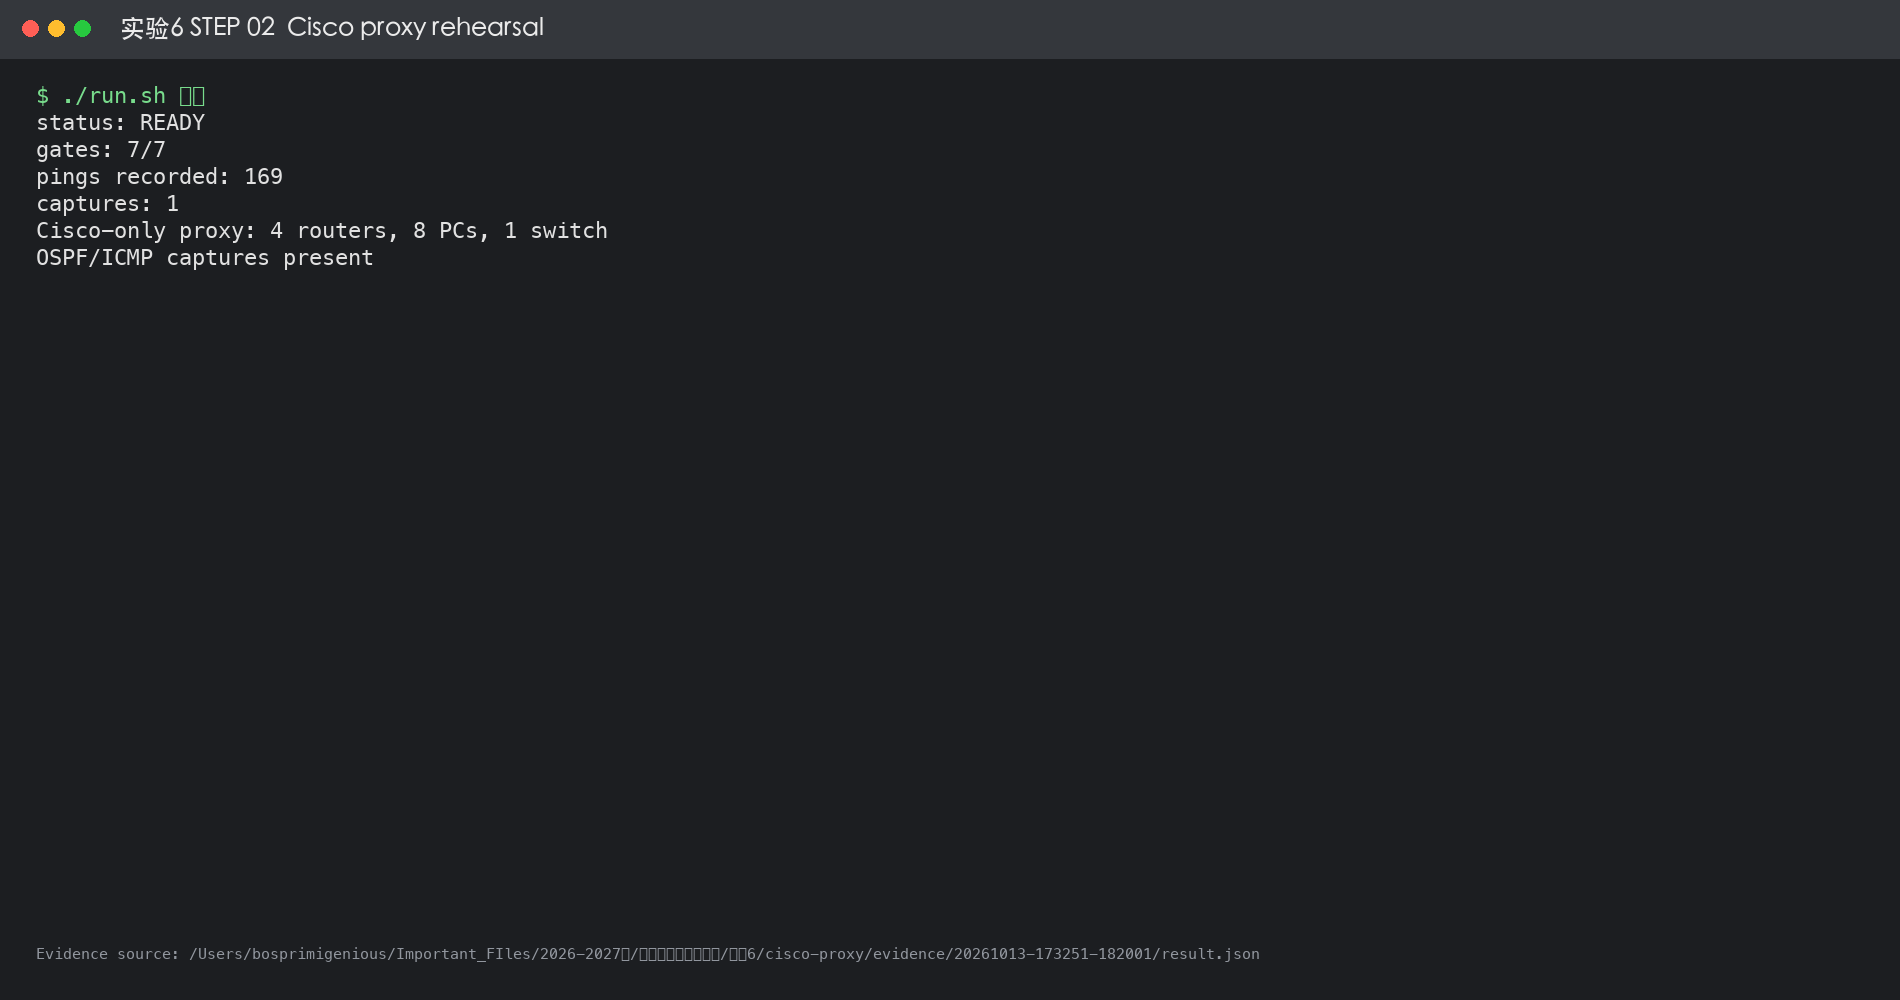
\includegraphics[width=0.96\textwidth]{截图/02-Cisco预演.png}\caption{Cisco-only proxy的实际验收摘要。}\end{figure}
\section{三厂商阻塞与结论}
真实验收result.json显示配置生成成功，但所有远端端点host为null，real\_three\_vendor门禁为false并返回2。当前没有Juniper/H3C镜像或实验室连接信息，因此实验六总体NOT READY。取得合法镜像或12个console端点后，先部署并手工确认接口，再运行verify\_remote.py。
\begin{figure}[H]\centering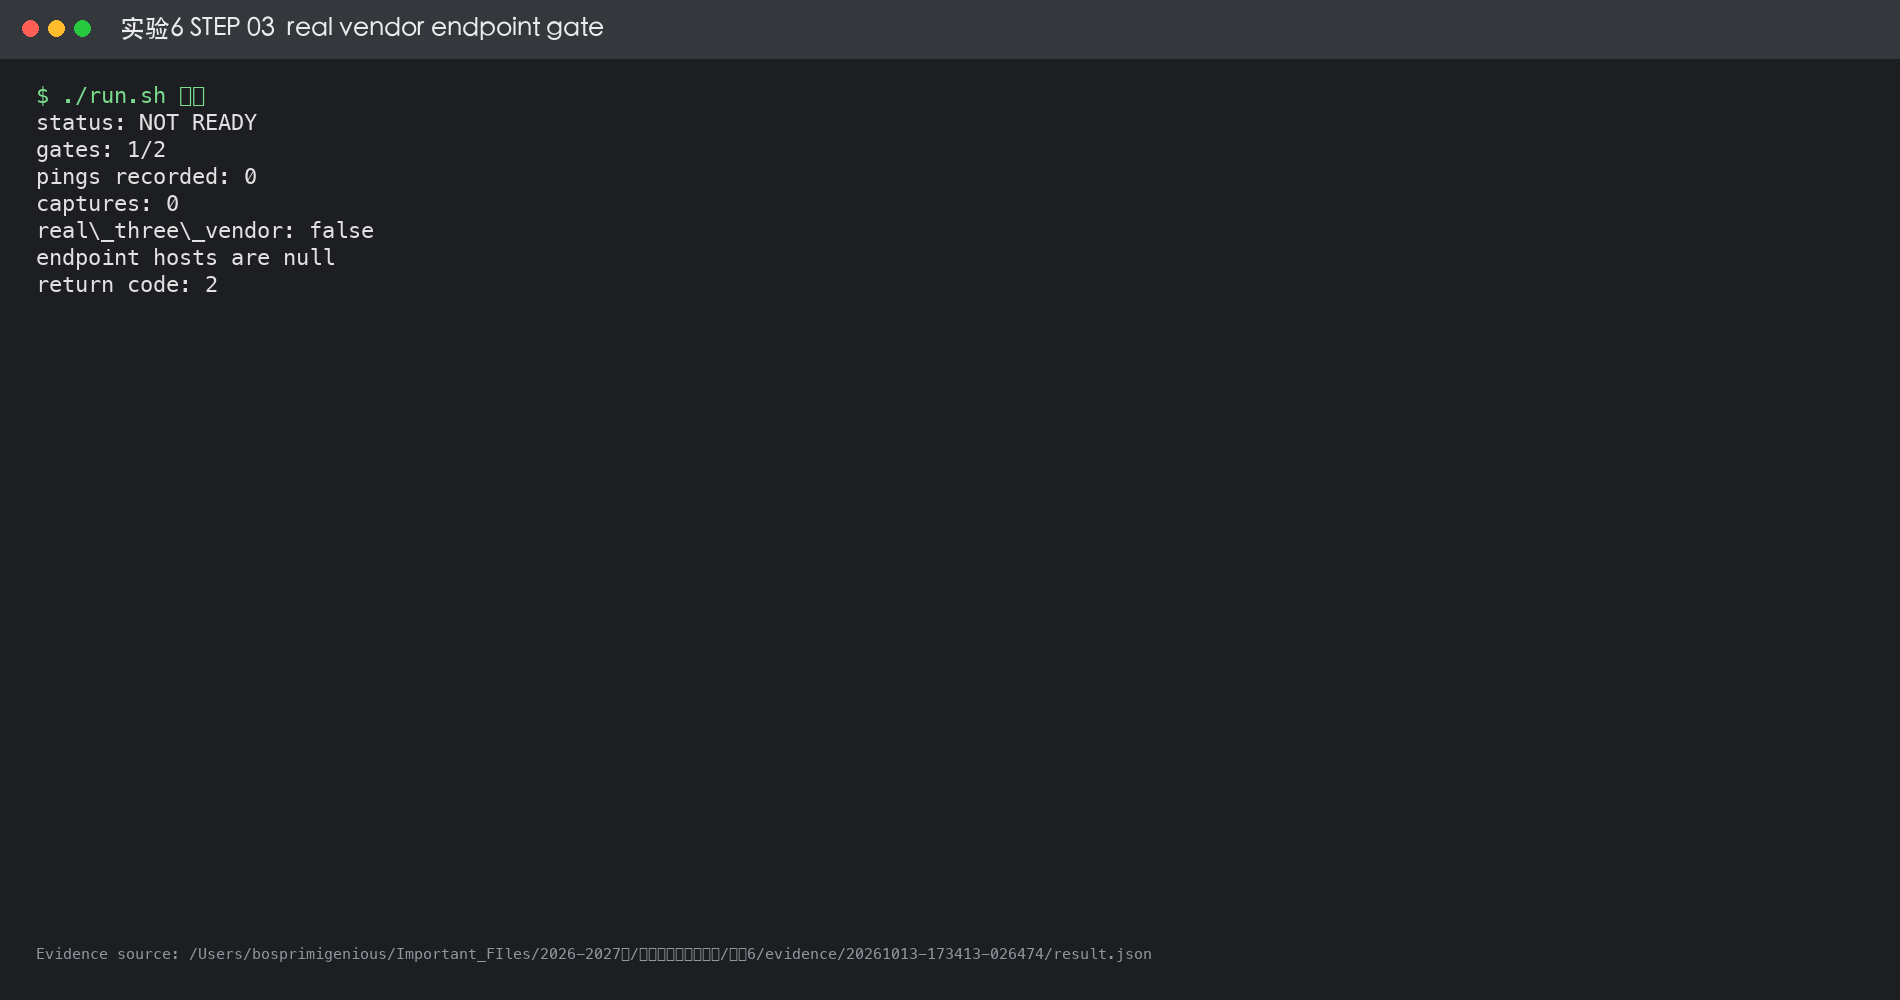
\includegraphics[width=0.96\textwidth]{截图/03-三厂商验收.png}\caption{真实三厂商端点缺失的硬阻塞。}\end{figure}
\section{截图与证据边界}
本报告的终端图由本项目实际Dynamips/Cisco IOS运行日志和验收JSON生成，原始证据目录保留在本实验的\texttt{evidence/}中。截图展示命令与回显，不把上游报告结果当作本实验结果。当前状态为\textbf{NOT READY}。
\section{结论}
本实验的拓扑、命令和部分阶段已经实现，但存在未通过门禁或外部环境阻塞；本报告记录当前证据，不能将其表述为完整通过。

\end{document}
